As specified in the call for the Lise-Meitner Fellowship the project plan is aligned for a duration of 24~months. The project is divided into five tangible \glspl{wp} of varying duration (Fig.~\ref{fig:flowchart}). \gls{wp}0 (Management and mentoring) and \gls{wp}5 (Reporting and dissemination) are designed to run through the whole project duration of 24~months concomitantly (Fig.~\ref{fig:ganttchart}).

\gls{wp}0 oversees the whole project and is central for the career development guided by the host institution. \gls{wp}0 has also a bi-directional component as mentoring and support is received by the applicant as well as given through co-supervision of master and PhD students. All communication, e.g. regular reporting to the \gls{fwf} and dissemination in the form of research papers, conference contributions, and public outreach activities, are bundled in \gls{wp}5. The scientific and technical work is assigned to \glspl{wp}~1--4. The technicality of the \glspl{wp} is decreasing from \gls{wp}1 (mainly technical) to \gls{wp}4 (purely scientific) with expected increasing scientific throughput. \gls{wp}1 (Model integration) and \gls{wp}2 (Model coupling) are tightly interlinked with \gls{wp}3 (Model evaluation) spanning the whole duration of \gls{wp}1 and \gls{wp}2. \gls{wp}2 depends on the realisation of \gls{wp}1, and \gls{wp}4 depends on the completion of all previous substantial \glspl{wp}~1--3. Each \gls{wp} has companion \glspl{ms} assigned. Further details on these \gls{ms} are presented in Section~\ref{sec:milestones}.\\

\begin{figure}[!ht]
  \centering
  %\subbottom[Flow chart]{%
    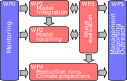
\includegraphics[width=0.75\textwidth]{wp_flow_chart}
    \caption{Flow chart of the \gls{odina} project, with \glspl{wp} as presented in this Section. All \glspl{wp} are embedded in \gls{wp}0 which coordinates the subordinate \glspl{wp}. \gls{wp}1 and \gls{wp}2 comprise the most technical aspects: integration of the \gls{odina} model into the \gls{clm}, coupling of \gls{odina} to the \gls{cam}-chem, and improvement of the dry deposition scheme. \gls{wp}2 is accompanied by a research stay at the \gls{ncar/ucar} lab in Boulder, \acrshort{col}, \acrshort{usa}. The \gls{wp}3 focuses on the evaluation of the \gls{odina} model performance. \gls{wp}4 comprises the production and analysis of long-term simulations (\gls{cmip}~6 style) and their comparison to available \gls{cesm} baseline simulations. \gls{wp}5 communicates an reports results continuously.}
  \label{fig:flowchart}%}\\
  \vspace{-1\baselineskip}
\end{figure}

Prof.~Rieder and members of his research group will support Dr.~Falk in all scientific, technical, and administrative matters of the \gls{odina} project. Individual contributions of the team members to \gls{odina} are specified below.\\

Prof.~Rieder will act as mentor to Dr.~Falk within \gls{odina}. He will devote 10\% of his time as in-kind support distributed across all \glspl{wp}. He will provide guidance on all scientific aspects of the project, the dissemination of results to scientific and lay audiences, and the advising and mentoring of students (PhD and MSc). Most importantly however, he will provide career counseling and support Dr.~Falk in growing her professional network, international, nationally and at the host institution, as well as assist her in developing and refining her leadership philosophy. Prof.~Rieder will also provide guidance regarding the selection of different trainings for staff development offered by \gls{boku} and make recommendations for additional courses or workshops offered by scientific unions or third-party providers. Further details on the mentor-mentee relationship are detailed in the career development plan in \hyperref[appendix:career]{Annex 3}.

Dr.~Alexander will support Dr.~Falk in all matters related to scientific computing. He will assist in model porting, model architecture and \gls{hpc} on the \gls{vsc} and in-house \gls{hpc} infrastructure. He will devote 10\% of his time as an in-kind contribution to \gls{odina}, distributed on \glspl{wp}~1,~2,~and~4. 

Dr.~Mayer will support Dr.~Falk in \glspl{wp}~1, 3, 4, and 5. Particularly, she will contribute to model evaluation and analyses tailored to quantify effects of two-way coupled ozone dry deposition on ambient air quality and plant health. She will devote 10\% of her time as an in-kind contribution to \gls{odina} and act as mentor to Dr.~Falk.    

Mr.~Staehle, Msc, is a PhD student in the Rieder group focusing on the climate-air quality-health nexus. His research is supported by institutional funds of \gls{boku}. He will contribute 50\% of his time as in-kind support to the \gls{odina} project, particularly \glspl{wp}~3--5. He will be jointly supervised on this research by Dr.~Falk and Prof.~Rieder.

Mrs.~Hasenhündl and Mrs.~Falmbigl are the administrative assistants of the host institute. They will support Dr.~Falk in all administrative matters during the course of the \gls{odina} project as well as during the preparation and the relocation phase upon receipt of the funding notice.\\

The host institute will provide all infrastructure necessary for a seamless implementation of the \gls{odina} project. This includes access to the national \gls{hpc} resources at \gls{vsc}, including private nodes and state-of-the-art storage and post-processing servers in-house at \gls{boku}. Upon approval of the \gls{odina} project Prof.~Rieder and Dr.~Alexander will assist Dr.~Falk in an application to obtain additional core hours on \gls{vsc} for \gls{odina}, which are commonly granted on basis of the operator agreement regarding peer-reviewed projects that require large computational resources. \gls{boku} will provide further office space, desktop \acrshort{it} equipment, and access to libraries and other university facilities. 

\vspace{-0.5\baselineskip}
\section{WP0 Management \& mentoring}
\label{sec:wp0}
The management and mentoring \gls{wp}, spans the entire project period and includes a variety of bi-directional tasks in cooperation and with support of the faculty host and host institute at \gls{boku}. \gls{wp}0 is built upon the core attributes of the Lise-Meitner Fellowship and shall enable the applicant to position herself as an emerging leader in land-atmosphere interactions, particularly the climate-vegetation-air quality nexus. During the start phase of the \gls{odina} project, \gls{wp}0 will ensure a smooth integration into the work environment at the host institute and involves all aspects concerning technical, administrative and logistic support by the corresponding units of \gls{boku} (\ref{itm:start}). The mid-phase is split into the development and honing of key skills for a future leadership role in Earth science (\ref{itm:career_dev}) and monitoring of the project progress (\ref{itm:progress}). \ref{itm:career_dev} includes leadership and management training but also programs focusing on didactic skills, presentation techniques, public outreach formats, as well as co-supervision of students. A detailed career development plan is presented in \hyperref[appendix:career]{Annex 3}. In the end-phase \gls{wp}0 will initiate the preparation of follow-up proposals tailored to European and national funding schemes such as e.g. the \gls{fwf} Elise Richter Program or Stand-Alone projects (\ref{itm:followup}).

\vspace{-0.5\baselineskip}
\subsection*{Work Package duration 24 months (months 1 to 24)}
\begin{enumerate}[start=1,label={T0.\arabic*}]
  \itemsep0pt
\item Setup and project start \hfill [month 1]\label{itm:start}
\item Career development \hfill [month 1 -- 24]\label{itm:career_dev}
\item Progress monitoring \hfill [month 1 -- 23]\label{itm:progress}
\item Follow-up projects \hfill [month 18 -- 24]\label{itm:followup}
\end{enumerate}

\vspace{-1\baselineskip}
\section{WP1 Model integration}
\label{sec:wp1}
The model integration \gls{wp} will build on existing collaborations with technical and scientific staff at the \gls{uio} (Norway) and at \gls{ncar/ucar} in Boulder (\acrshort{col}, \acrshort{usa}) and include support by the scientific and technical team of the host institute at \gls{boku}, Vienna. Existing parts of the \gls{odina} model will be extended to describe our process understanding as accurately as possible. This will comprise
\begin{enumerate}
  \itemsep0pt
\item to include a state of stomata sluggishness and take a more explicit healing formulation into consideration (\ref{itm:slugg}) and
\item to deduce and update additional model parameters based on existing databases (\ref{itm:para}).
\end{enumerate}
It is expected that the model output considering active ozone damage will substantially differ between the updated (this proposal) and current \gls{cesm} configuration (\gls{cmip}~6). Initial cross-evaluation with data at global scales (coarse resolution model integration) and single site simulations (\ref{itm:init_sim}) following the \gls{cesm} standard procedures are likely to reveal the necessity for adjustment of additional free model parameters. An in-depth evaluation of individual parameters and results is subject to \gls{wp}3.

\vspace{-0.5\baselineskip}
\subsection*{Work Package duration 4 months (months 1 to 4)}
\begin{enumerate}[start=1,label={T1.\arabic*}]
  \itemsep0pt
\item Implementation of stomatal sluggishness and healing \hfill [month 1 -- 2]\label{itm:slugg}
\item Deduction of additional parameters \hfill [month 2 -- 3]\label{itm:para}
\item Initial model simulations and cross-evaluation \hfill [month 3 -- 4]\label{itm:init_sim}
\end{enumerate}

\section{WP2 Model coupling}
\label{sec:wp2}
Activities related to model coupling will include an extended research stay at the \gls{ncar/ucar} lab in Boulder (\acrshort{col}, \acrshort{usa}) to both facilitate the technical work as well as build important networks for future research activities. A one-way coupling between the atmospheric chemistry component (e.g. \gls{cam}-chem) to the land-surface component (\gls{clm}) is achieved through the dry deposition implementation already in place in \gls{cesm}. The existing dry deposition scheme in \gls{cesm} will be evaluated concerning \gls{odina}. If necessary, the scheme will be improved and updated (\ref{itm:drydep}). Two-way coupling will be achieved by propagating instantaneous ozone concentrations from the atmosphere through the coupler to the land component (\ref{itm:couple}). Technically this involves touching the \gls{cesm} coupler infrastructure. The work on the coupling will be done in the most sustainable way during the planned research stay at \gls{ncar/ucar}. Potential infrastructure updates will be taken into consideration and integrated into the workflow. Initial tests and evaluation of the coupled model on coarse-grid global-scale as well as through single site simulations are planned (\ref{itm:couple_test}). Detailed evaluation of the coupled model performance will be pursued in coordination with \gls{wp}3.
{
\subsection*{Work package duration 5 months (months 4 to 8)}
\begin{enumerate}[start=1,label={T2.\arabic*}]
  \itemsep0pt
\item Evaluation of the dry deposition scheme (improvement and update) \hfill [month 4 -- 5]\label{itm:drydep}
\item Technically coupling \gls{cam}-chem ozone concentrations to \gls{odina} \\$\rightarrow$ research stay at \gls{ncar/ucar} \hfill [month 5 -- 6]\label{itm:couple}
\item Perform model tests of the coupling algorithm \hfill [month 6 -- 8]\label{itm:couple_test}
\end{enumerate}
}

\section{WP3 Model evaluation \& update of model parameters}
\label{sec:wp3}
The evaluation of the updated model is an integral part of \gls{wp}1 and \gls{wp}2 and spans the whole duration of both \glspl{wp}. Data for evaluation will be collected from Fluxnet sites with associated ground level ozone observations, e.g. the \gls{airbase} (\ref{itm:eval_data}). Based on the collected data, the initial integration and validation tests are complemented and completed with more in depth evaluation for the selected sites (\ref{itm:eval_site}) and on global scales (\ref{itm:eval_glob}). In conjunction with \ref{itm:eval_site} the project team will work closely with the \gls{clm} team Norway at \gls{uio}. This will utilize also the land-modelling platform developed in collaboration with the applicant during her PostDoc at \gls{uio}. Variable model parameters will be adapted and adjusted if necessary to further improve the resulting model skills in terms of, e.g. \gls{npp}/\gls{gpp} (\ref{itm:update_para}). A model development and evaluation paper is pursued in coordination with \gls{wp}5.
{
\subsection*{Work Package duration 11 months (months 1 to 11)}
\begin{enumerate}[start=1,label={T3.\arabic*}]
  \itemsep0pt
\item Collection of evaluation data \hfill [month 1 -- 3]\label{itm:eval_data}
\item Site level evaluation \hfill [month 3 -- 6]\label{itm:eval_site}
\item Global scale evaluation \hfill [month 6 -- 11]\label{itm:eval_glob}
\item Update model parameters \hfill [month 3 -- 11]\label{itm:update_para}
\end{enumerate}
}

\vspace{0.5\baselineskip}
\section{WP4 Production runs \& future projections}
\label{sec:wp4}
Upon successful implementation of \gls{wp}~1--3 work on \gls{wp}4 is initiated. Within this final research \gls{wp} production runs with climate projections will be performed. It is planned to perform at least one long-term \gls{cmip} style ($1850-2100$) coupled model simulation (\ref{itm:ssp5}). As the highest tropospheric ozone abundances are expected for a low mitigation scenario with high anthropogenic greenhouse gas emissions and simultaneous substantial methane release from permafrost regions \parencites[e.g.][]{JGR:Rieder2015}{AE:Rieder2018}, \gls{ssp}~5 is selected as a future scenario. Additional simulations following other \glspl{ssp} are planned but completion will depend on the workload of the \gls{vsc} and thus cannot be guaranteed to be fully achieved within the 24~month project timeline. Of special interest are implications on future surface ozone abundance and air quality indices (\ref{itm:eval_ozone}) along with induced plant damage and effects on the carbon cycle (\ref{itm:eval_clim}), e.g. expected reduction in \gls{gpp} with respect to reference simulations. The focus herein lies on populous and highly industrialized regions, e.g. Europe, East Asia, North America. To quantify the effects on carbon sequestration and climate, long-term simulations with the updated \gls{cesm} for comparison with existing \gls{cmip}~6 simulations will be conducted. Two scientific papers are expected to emerge out of \gls{wp}4, one focusing on future ozone air quality the other on ozone related plant damage.
{
\subsection*{Work Package duration 14 months (months 11 to 24)}
\begin{enumerate}[start=1,label={T4.\arabic*}]
  \itemsep0pt
\item Coupled \gls{cesm} simulation on climatological timescales (\gls{ssp}5) \hfill [month 11 -- 17]\label{itm:ssp5}
\item Evaluate climate and vegetation impacts on surface ozone abundance \hfill [month 11 -- 17]\label{itm:eval_ozone}
\item Quantify the effects on carbon sequestration and climate forcing. \hfill [month 17 -- 24]\label{itm:eval_clim}
\end{enumerate}
}

%\vspace{0.5\baselineskip}
\section{WP5 Reporting \& dissemination}
\label{sec:wp5}
\gls{wp}5 acts as an umbrella for reporting to the funding agency (\gls{fwf}) and dissemination to scientific and lay audiences. \gls{wp}5 spans the whole project duration and is effectively the coordinating and reporting hub for \gls{wp}1--4. Science communication (\ref{itm:communication}) is further divided into research papers, conference contributions, and public outreach. 
At least three research papers are expected to emerge out of the \gls{odina} project, one focusing on model development and evaluation, one on future changes in ambient air quality and one on ozone induced plant damage and effects on the carbon cycle.
Public outreach will include among others contributions to popular science blogs or presentations to the general public. Dissemination using social media platforms such as twitter will be considered if applicable. In close interaction with \gls{wp}0 and under guidance by the host institution, targeted networking activities are planned (e.g. conferences, workshops, professional networks) (\ref{itm:networking}). The submission of the final report to the funding agency (\gls{fwf}) is officially concluding \gls{wp}5 (\ref{itm:prep_reports}) although several additional papers are expected to emerge from the project past official completion.
{
\subsection*{Work Package duration 24 months (months 1 to 24)}
\begin{enumerate}[start=1,label={T5.\arabic*}]
  \itemsep0pt
\item Science communication \hfill [month 3 -- 24]\label{itm:communication}
\item Networking \hfill [month 1 -- 24]\label{itm:networking}
\item Prepare annual reports to funding agency (\gls{fwf}) \hfill [month 12 / 24]\label{itm:prep_reports}
\end{enumerate}
}

\vspace{0.5\baselineskip}
\section{Milestones}
\label{sec:milestones}
Each \gls{wp} has companion \glspl{ms} assigned. In Fig.~\ref{fig:ganttchart}, the colored bars represent the \glspl{wp} while the \glspl{ms} are denoted with a star. \gls{ms}0a marks the mid-term evaluation of the Lise-Meitner Fellowship program, while its completion is denoted by \gls{ms}0b. \gls{ms}1--3 mark the successful completion of \gls{wp}1--3, respectively. \gls{ms}4a marks the completion of the long-term \gls{cmip}~6 style simulations and is followed by the completion of the assessment and analysis of the model results (\gls{ms}4b) regarding impacts of the updated \gls{cesm} on air quality and climate. \gls{ms}5 comprises the annual reporting to the \gls{fwf} (2~reports).

\begin{enumerate}[start=0,label={MS\arabic*}]
  \itemsep0pt
  \item
  \begin{enumerate}[a]
  \item Mid-term evaluation of the career development and mentoring program \ \hfill [month 12]
  \item Completion of career development and mentoring program \hfill [month 24]
  \end{enumerate}
\item \quad Completion of model integration \hfill [month 4]
\item \quad Completion of model component coupling \hfill [month 8]
\item \quad Completion of initial model simulations and cross-evaluation \hfill [month 11]
\item 
\begin{enumerate}[a]
    \item Completion of model long-term \gls{cmip}~6 style simulations \hfill [month 17]
    \item Completion of analysis of \gls{cesm} long-term simulations \hfill [month 20]
\end{enumerate}
\item 
  \begin{enumerate}[a]
  \item Research article submission \hfill [month 13 / 22 / 24]
  \item Annual reports to funding agency (\gls{fwf}) \hfill [month 12 / 24]
  \end{enumerate}
\end{enumerate}

\begin{figure}[!ht]
  \centering
  %\subbottom[Gantt chart]
   %\vspace{-30pt}
\end{figure}

